\PassOptionsToPackage{hyphens}{url}
\documentclass[superscriptaddress, nofootinbib,  amsmath, amssymb, twocolumn]{revtex4-2}

\usepackage[margin=1.5cm]{geometry} 
\usepackage[english]{babel}
\usepackage[utf8]{inputenc}
\usepackage[]{graphicx}
\usepackage{xspace}
\usepackage{siunitx}
\usepackage{mhchem}
\DeclareSIUnit\angstrom{\text {Å}}
\usepackage{orcidlink}
\usepackage{hyperref}
\usepackage{fontawesome5}
\usepackage{natmove}
\usepackage{placeins}

\usepackage{xparse}
\usepackage{hyperref}
\usepackage[a-1b]{pdfx}

\newcommand{\githublink}[2]{
  \href{https://github.com/#1/#2}{\faGithub\ \url{#1/#2}}
}

\newcommand{\twitterlink}[1]{
  \href{#1}{\faTwitter}
}

\newcommand{\zenodolink}[1]{
  \href{https://doi.org/#1}{\faArchive\ \url{#1}}
}

%https://twitter.com/SamCox822/status/1641484192566460416?s=20


\newcommand{\hflogo}{%

\includegraphics[height=.9em]{figures/huggingface.png}
}

\newcommand{\huggingfacelink}[2]{
  \href{https://huggingface.co/spaces/#1/#2}{\hflogo \url{#1/#2}}
}

\newcommand{\huggingfacehublink}[2]{
  \href{https://huggingface.co/#1/#2}{\hflogo \url{#1/#2}}
}

% Adjusted Hyperref Setup for Automatically Colored Text Links
\hypersetup{
  colorlinks=true,       % Enables colored links
  breaklinks=true,
  urlcolor=blue,         % Sets the color of URL links
  linkcolor=blue,        % Sets the color of internal links
  citecolor=blue,        % Sets the color of citation links
  filecolor=blue,        % Sets the color of file links
  allcolors=blue,        % Ensures all link types are blue by default
  pdftitle={Title},      % PDF Title
  pdfauthor={Author}     % PDF Author
}

\usepackage[nameinlink,capitalise]{cleveref} %needs to appear after hyperref, https://tex.stackexchange.com/questions/396728/my-equations-referencing-not-working
\Crefname{figure}{Figure}{Figures} %needs to appear after hyperref and cleveref
\crefname{appsec}{Appendix}{Appendices}
\newcommand\crefrangeconjunction{--} % modify the reference style


% =====================================================
% packages for creating code listings 
\usepackage{listings, xcolor}
\definecolor{codegreen}{rgb}{0,0.6,0}
\definecolor{codegray}{rgb}{0.5,0.5,0.5}
\definecolor{codepurple}{rgb}{0.58,0,0.82}
\definecolor{tqblue}{HTML}{08293d}
\definecolor{backcolour}{HTML}{fefdf5}

\lstdefinestyle{pythonstyle}{
    backgroundcolor=\color{backcolour},   
    commentstyle=\color{codegreen},
    keywordstyle=\color{magenta},
    numberstyle=\tiny\color{codegray},
    stringstyle=\color{codepurple},
    basicstyle=\ttfamily\footnotesize\color{tqblue},
    breakatwhitespace=false,         
    breaklines=true,
    postbreak=\mbox{\textcolor{magenta}{$\hookrightarrow$}\space},                 
    captionpos=b,                    
    keepspaces=true,                 
    numbers=left,                    
    numbersep=5pt,                  
    showspaces=false,                
    showstringspaces=false,
    showtabs=false,                  
    tabsize=2
}

\lstset{style=pythonstyle}
\hbadness=99999 

\newcolumntype{C}{>{$}c<{$}}

\AtBeginDocument{%
  \heavyrulewidth=.08em
  \lightrulewidth=.05em
  \cmidrulewidth=.03em
  \belowrulesep=.65ex
  \belowbottomsep=0pt
  \aboverulesep=.4ex
  \abovetopsep=0pt
  \cmidrulesep=\doublerulesep
  \cmidrulekern=.5em
  \defaultaddspace=.5em
}



\usepackage[most]{tcolorbox}

\tcbset {
  base/.style={
    arc=0mm, 
    bottomtitle=0.5mm,
    boxrule=0mm,
    colbacktitle=black!10!white, 
    coltitle=black, 
    fonttitle=\bfseries, 
    left=2.5mm,
    leftrule=1mm,
    right=8.5mm,
    title={#1},
    toptitle=0.75mm, 
    width=\textwidth,
    breakable
  }
}

\definecolor{brandblue}{rgb}{0, 0.27843137254902, 0.466666666666667}
\newtcolorbox{agentinteraction}[1]{
  colframe=brandblue, 
  base={#1}
}


\definecolor{brandbred}{rgb}{0.63921568627451, 0, 0}
\newtcolorbox{agentinteraction2}[1]{
  colframe=brandbred, 
  base={#1}
}


\newtcolorbox{subbox}[1]{
  colframe=black!30!white,
  base={#1}
  }

\usepackage [autostyle, english = american]{csquotes}
\usepackage[acronym, nonumberlist]{glossaries}
\makeglossaries

\newacronym{llm}{LLM}{large language model}
\newacronym{gpt}{GPT}{generative pretrained transformer}
\newacronym{api}{API}{application programming interface}
\newacronym{ml}{ML}{machine learning}
\newacronym{lift}{LIFT}{language-interfaced fine-tuning}
\newacronym{icl}{ICL}{in-context learning}
\newacronym{peft}{PEFT}{parameter efficient fine-tuning}
\newacronym{lora}{LoRA}{low-rank adaptors}
\newacronym{gpr}{GPR}{Gaussian process regression}
\newacronym{ga}{GA}{genetic algorithm}
\newacronym{svm}{SVM}{support vector machine}
\newacronym{rf}{RF}{random forest}

\newacronym{ord}{ORD}{Open Reaction Database}
\newacronym{bo}{BO}{Bayesian optimization}
\newacronym{id}{ID}{inverse design}
\newacronym{mad}{MAD}{median absolute deviation}
\newacronym{eln}{ELN}{electronic lab notebook}
\newacronym[shortplural=LIMS]{lims}{LIMS}{laboratory information system}
\newacronym{ui}{UI}{user interface}
\newacronym{nlm}{NLM}{national library of medicine} 
\newacronym{dft}{DFT}{density functional theory}
\newacronym{cot}{COT}{chain of thought}
\newacronym{gui}{GUI}{graphical user interface}
\newacronym{pdb}{PDB}{protein data bank}
\newacronym{rlhf}{RLHF}{reinforcement learning from human feedback}
\newacronym{json}{JSON}{JavaScript object notation}
\newacronym{smiles}{SMILES}{simplified molecular-input line-entry system}
\newacronym{selfies}{SELFIES}{self-referencing embedded strings}
\newacronym{ai}{AI}{artificial intelligence}
\newacronym{nlp}{NLP}{natural language processing}
\newacronym{ner}{NER}{named entity recognition}
\newacronym{cas}{CAS}{Chemical Abstract Services}
\newacronym{mae}{MAE}{mean absolute error}
\newacronym{inchi}{InChI}{international chemical identifier}
\newacronym{mapi}{MAPI}{Materials Project \gls{api}}
\newacronym{rouge}{ROUGE}{Recall-Oriented Understudy for Gisting Evaluation}
\newacronym{html}{HTML}{HyperText Markup Language}
\newacronym{doi}{DOI}{digital object identifier}
\newacronym{ocr}{OCR}{optical character recognition}

\usepackage{tabularx} % For flexible tables with adjustable column widths
\usepackage{booktabs} % For better table lines (\toprule, \midrule, \bottomrule)
\usepackage{cleveref}

\let\originalcite\cite
\renewcommand{\cite}[1]{\unskip~\originalcite{#1}}

\usepackage{setspace}

% \clubpenalty=10000
% \widowpenalty=10000
% \displaywidowpenalty=10000
\usepackage{titlesec}

\titlespacing{\subsection}
    {0pt}{9pt}{6pt}

\usepackage{array}
\usepackage{ragged2e}
\usepackage{nicefrac}
\usepackage[caption=false]{subfig}

\newcolumntype{P}[1]{>{\raggedright\arraybackslash}p{#1}}

\begin{document}

\title{Bayesian Optimization Hackathon for Chemistry and Materials}

% %ToDo: add contributed equally indication for participants

\newcommand{\equalcont}{\thanks{These authors contributed equally}}

\author{Kevin~Maik~Jablonka~\orcidlink{0000-0003-4894-4660}}
\email{mail@kjablonka.com}
\affiliation{Laboratory of Molecular Simulation (LSMO), Institut des Sciences et Ing\'{e}nierie Chimiques, Ecole Polytechnique F\'{e}d\'{e}rale de Lausanne (EPFL), Sion, Valais, Switzerland.}

\author{Qianxiang Ai~\orcidlink{0000-0002-5487-2539}}
\equalcont
\affiliation{Department of Chemical Engineering, Massachusetts Institute of Technology, Cambridge, Massachusetts 02139, United States.}

%\email{qai@mit.edu}


\author{Alexander~Al-Feghali~\orcidlink{0009-0004-8377-7049}} 
\equalcont
%\email{alexander.al-feghali@mail.mcgill.ca}
\affiliation{Department of Chemistry, McGill University, Montreal, Quebec, Canada.}

\author{Shruti~Badhwar~\orcidlink{0000-0002-3167-5348}}
\equalcont
\affiliation{Reincarnate Inc.}  
%\email{shruti@reincarnateartificial.com}

\author{Joshua~D.~Bocarsly~\orcidlink{0000-0002-7523-152X}}
\equalcont
 \affiliation{Yusuf Hamied Department of Chemistry, University of Cambridge, Lensfield Road, Cambridge, CB2 1EW, United Kingdom.} 
 
%\email{jb2382@cam.ac.uk} 

\author{Andres~M~Bran~\orcidlink{0000-0002-4432-3667}}
\equalcont
\affiliation{Laboratory of Artificial Chemical Intelligence (LIAC), Institut des Sciences et Ing\'{e}nierie Chimiques, Ecole Polytechnique F\'{e}d\'{e}rale de Lausanne (EPFL), Lausanne, Switzerland.} 
\affiliation{National Centre of Competence in Research (NCCR) Catalysis, Ecole Polytechnique F\'{e}d\'{e}rale de Lausanne (EPFL), Lausanne, Switzerland.}


\author{Stefan~Bringuier~\orcidlink{0000-0001-6753-1437}}
\equalcont
\affiliation{Independent Researcher, San Diego, CA, United States.}
%\email{stefanbringuier@gmail.com}

\author{L.~Catherine~Brinson~\orcidlink{0000-0003-2551-1563}}
\equalcont
\affiliation{Mechanical Engineering and Materials Science, Duke University, United States.}
%\email{cate.brinson@duke.edu}



\author{Defne~Circi~\orcidlink{0000-0002-5761-0198}}
\equalcont
\affiliation{Mechanical Engineering and Materials Science, Duke University, United States.}
%\email{defne.circi@duke.edu}

\author{Sam~Cox~\orcidlink{0000-0002-4441-9327}}
\equalcont
\affiliation{Department of Chemical Engineering, University of Rochester, United States.}
%\email{swrig30@ur.rochester.edu}

\author{Wibe~A.~de~Jong~\orcidlink{0000-0002-7114-8315}} 
\equalcont
\affiliation{Applied Mathematics and Computational Research Division, Lawrence Berkeley National Laboratory, Berkeley, CA 94720, United States.
}

\author{Matthew~L.~Evans~\orcidlink{0000-0002-1182-9098}}
\equalcont
 \affiliation{Institut de la Matière Condensée et des Nanosciences (IMCN), UCLouvain, Chemin des Étoiles 8, Louvain-la-Neuve, 1348, Belgium.}
 \affiliation{Matgenix SRL, 185 Rue Armand Bury, 6534 Gozée, Belgium.}
 %\email{matthew.evans@uclouvain.be}

 \author{Nicolas~Gastellu~\orcidlink{0000-0002-4052-076X}}
 \equalcont
\affiliation{Department of Chemistry, McGill University, Montreal, Quebec, Canada.}
%\email{nicolas.gastellu@mail.mcgill.ca} 

\author{Jerome~Genzling~\orcidlink{0009-0007-4728-1478}} 
\equalcont
\affiliation{Department of Chemistry, McGill University, Montreal, Quebec, Canada.}
%\email{jerome.genzling@mail.mcgill.ca}

\author{Mar\'ia~Victoria~Gil~\orcidlink{0000-0002-2258-3011}}
\equalcont
\affiliation{Instituto de Ciencia y Tecnolog\'ia del Carbono (INCAR), CSIC, Francisco Pintado Fe 26, 33011 Oviedo, Spain.}
%\email{victoria.gil@incar.csic.es}

\author{Ankur~K.~Gupta~\orcidlink{0000-0002-3128-9535}}
\equalcont
\affiliation{Applied Mathematics and Computational Research Division, Lawrence Berkeley National Laboratory, Berkeley, CA 94720, United States.
}


\author{Alishba~Imran}
\equalcont
\affiliation{Computer Science, University of California, Berkeley, Berkeley CA 94704, United States.}

\author{Sabine~Kruschwitz~\orcidlink{0000-0002-6296-4417}}
\equalcont
\affiliation{Bundesanstalt für Materialforschung und -prüfung, Unter den Eichen 87, 12205 Berlin, Germany.}
%\email{Sabine.Kruschwitz@bam.de}

\author{Anne~Labarre~\orcidlink{0000-0003-4939-3928}}
\equalcont
\affiliation{Department of Chemistry, McGill University, Montreal, Quebec, Canada.}
 %\email{Anne.Labarre@mail.mcgill.ca}  

\author{Jakub~Lála~\orcidlink{0000-0002-5424-5260}}
\equalcont
\affiliation{Francis Crick Institute, 1 Midland Rd, London NW1 1AT, United Kingdom.}
%\email{jakublala@gmail.com}
 
\author{Tao~Liu~\orcidlink{0000-0002-1082-5570}}
\equalcont
\affiliation{Department of Chemistry, McGill University, Montreal, Quebec, Canada.}
 %\email{tao.liu7@mail.mcgill.ca} 

\author{Steven~Ma~\orcidlink{0000-0006-9448-7332}}
\equalcont
\affiliation{Department of Chemistry, McGill University, Montreal, Quebec, Canada.}
 %\email{Steven.Ma@mail.mcgill.ca} 

\author{Sauradeep~Majumdar~\orcidlink{0000-0002-2095-3082}}
\equalcont
\affiliation{Laboratory of Molecular Simulation (LSMO), Institut des Sciences et Ing\'{e}nierie Chimiques, Ecole Polytechnique F\'{e}d\'{e}rale de Lausanne (EPFL), Sion, Valais, Switzerland.}
%\email{sauradeep.majumdar@epfl.ch}

\author{Garrett~W.~Merz~\orcidlink{0000-0003-4737-3931}}
\equalcont
\affiliation{American Family Insurance Data Science Institute, University of Wisconsin-Madison, Madison WI 53706, United States.}


\author{Nicolas~Moitessier~\orcidlink{0000-0001-6933-2079}}
\equalcont
\affiliation{Department of Chemistry, McGill University, Montreal, Quebec, Canada.}
%;  Department of Chemistry, McGill University, Montreal, Quebec, Canada; orcid.org/; 
%\email{nicolas.moitessier@mcgill.ca}

\author{Elias~Moubarak~\orcidlink{0000-0001-8271-6800}}
\equalcont
\affiliation{Laboratory of Molecular Simulation (LSMO), Institut des Sciences et Ing\'{e}nierie Chimiques, Ecole Polytechnique F\'{e}d\'{e}rale de Lausanne (EPFL), Sion, Valais, Switzerland.}
%\email{elias.moubarak@epfl.ch}



\author{Beatriz~Mouriño~\orcidlink{0000-0003-1670-3985}}
\equalcont
\affiliation{Laboratory of Molecular Simulation (LSMO), Institut des Sciences et Ing\'{e}nierie Chimiques, Ecole Polytechnique F\'{e}d\'{e}rale de Lausanne (EPFL), Sion, Valais, Switzerland.}
%\email{beatriz.buenomourino@epfl.ch}

\author{Brenden~Pelkie~\orcidlink{0000-0001-7638-6366}}
\equalcont
\affiliation{Department of Chemical Engineering, University of Washington, Seattle, WA 98105, United States.} 
%\email{bgpelkie@uw.edu} 

\author{Michael~Pieler~\orcidlink{0000-0001-9186-7045}}
\equalcont
\affiliation{OpenBioML.org}
\affiliation{Stability.AI}
%\email{ michael.pieler@gmail.com}

\author{Mayk~Caldas~Ramos~\orcidlink{0000-0001-5336-2847}}
\equalcont
\affiliation{Department of Chemical Engineering, University of Rochester, United States.}
%\email{mcaldasr@ur.rochester.edu}

\author{Bojana~Ranković~\orcidlink{0000-0002-1476-6686}}
\equalcont
\affiliation{Laboratory of Artificial Chemical Intelligence (LIAC), Institut des Sciences et Ing\'{e}nierie Chimiques, Ecole Polytechnique F\'{e}d\'{e}rale de Lausanne (EPFL), Lausanne, Switzerland.}
\affiliation{National Centre of Competence in Research (NCCR) Catalysis, Ecole Polytechnique F\'{e}d\'{e}rale de Lausanne (EPFL), Lausanne, Switzerland.}


\author{Jacob~N.~Sanders~\orcidlink{0000-0002-2196-4234}}
\equalcont
\affiliation{Department of Chemistry and Biochemistry, University of California, Los Angeles, CA 90095, United States.}
%\email{jacosand@gmail.com}




\author{Philippe~Schwaller~\orcidlink{0000-0003-3046-6576}}
\equalcont
\affiliation{Laboratory of Artificial Chemical Intelligence (LIAC), Institut des Sciences et Ing\'{e}nierie Chimiques, Ecole Polytechnique F\'{e}d\'{e}rale de Lausanne (EPFL), Lausanne, Switzerland.}
\affiliation{National Centre of Competence in Research (NCCR) Catalysis, Ecole Polytechnique F\'{e}d\'{e}rale de Lausanne (EPFL), Lausanne, Switzerland.}

 
\author{Marcus~Schwarting}
\equalcont
 \affiliation{Department of Computer Science, University of Chicago, Chicago IL 60490, United States.}
 %\email{meschw04@uchicago.edu}


\author{Jiale~Shi~\orcidlink{0000-0002-5447-3925}}
\equalcont
\affiliation{Department of Chemical Engineering, Massachusetts Institute of Technology, Cambridge, Massachusetts 02139, United States.}
 %\email{jialele@mit.edu}
 
 \author{Berend~Smit~\orcidlink{0000-0003-4653-8562}}
%\email{berend.smit@epfl.ch}
\equalcont
\affiliation{Laboratory of Molecular Simulation (LSMO), Institut des Sciences et Ing\'{e}nierie Chimiques, Ecole Polytechnique F\'{e}d\'{e}rale de Lausanne (EPFL), Sion, Valais, Switzerland.}

\author{Ben~E.~Smith~\orcidlink{0000-0001-9673-2449}}
\equalcont
 \affiliation{Yusuf Hamied Department of Chemistry, University of Cambridge, Lensfield Road, Cambridge, CB2 1EW, United Kingdom.} 
%\email{bs542@cam.ac.uk} 


\author{Joren~Van~Herck~\orcidlink{009-0005-5108-5061}}
\equalcont
\affiliation{Laboratory of Molecular Simulation (LSMO), Institut des Sciences et Ing\'{e}nierie Chimiques, Ecole Polytechnique F\'{e}d\'{e}rale de Lausanne (EPFL), Sion, Valais, Switzerland.}
%\email{joren.vanherck@epfl.ch}


\author{Sean~Warren~\orcidlink{0000-0002-3670-0354}}
\equalcont
%\affiliation{}
%\email{sean.warren@gatech.edu}



\author{Sylvester~Zhang}
\equalcont
\affiliation{Department of Chemistry, McGill University, Montreal, Quebec, Canada.}

\author{Xiaoqi~Zhang\orcidlink{0000-0002-6507-6490}}
\equalcont
\affiliation{Laboratory of Molecular Simulation (LSMO), Institut des Sciences et Ing\'{e}nierie Chimiques, Ecole Polytechnique F\'{e}d\'{e}rale de Lausanne (EPFL), Sion, Valais, Switzerland.}
%\email{xiaoqi.zhang@epfl.ch}


\author{Ghezal~Ahmad~Zia~\orcidlink{0000-0002-9082-9423}} 
\equalcont
\affiliation{Bundesanstalt für Materialforschung und -prüfung, Unter den Eichen 87, 12205 Berlin, Germany.}
%\email{Ghezal-Ahmad.Zia@bam.de} 



% organiziers 

\author{KJ~Schmidt}
%\email{kj.schmidt913@gmail.com}
\affiliation{Globus, University of Chicago, Data Science and Learning Division, Argonne National Lab, United States.}

\author{Ian~Foster~\orcidlink{0000-0003-2129-5269}}
\affiliation{Department of Computer Science, University of Chicago, Data Science and Learning Division, Argonne National Lab, United States.}

\author{Ben~Blaiszik~\orcidlink{0000-0002-5326-4902}}
\email{blaiszik@uchicago.edu}
\affiliation{Globus, University of Chicago, Data Science and Learning Division, Argonne National Lab, United States.}








\begin{abstract}
The Acceleration Consortium and Merck KGaA hosted a 2-day virtual hackathon on March 27-28, 2024, bringing together scientists to explore, collaborate, and innovate in the field of Bayesian optimization for the physical sciences. Participants were encouraged to select or develop Bayesian optimization algorithms, apply them to benchmarking tasks, design new benchmarks, create instructional tutorials, and describe real-world applications. With over 100 participants across 60 academic, industry, and government organizations located in 38 cities, 14 countries, and 4 continents, this was a global event. % https://chatgpt.com/share/f6cd733f-1126-4151-86c5-d4b59d158dc3
The outputs from this event, including developed algorithms, benchmarks, and tutorials, will serve as valuable resources for the research community, in addition to the new skills learned and connections formed. Released projects and general information are available at \url{https://ac-bo-hackathon.github.io/} and other locations linked from individual project pages. This event demonstrated the potential of community-driven research efforts to accelerate advances in Bayesian optimization in chemistry and materials science.
\end{abstract}

\maketitle


% ToDo: 
% emphasize tooling/constrained prompting/guidance 

\section{Introduction}

Bayesian optimization (BO) has emerged as a powerful tool in optimizing complex and expensive-to-evaluate functions, often outperforming traditional search methods in a variety of scientific domains such as optimizing composition and processing parameters to maximize alloy yield strength or identifying synthesis pathways that maximize efficacy of HIV drugs (\cref{fig:intro-bo}). Hackathons help people to connect, gain skills, and flesh out new ideas. In the words of Michelle Duke, the "Hackathon Queen":

\begin{quote}
A hackathon is a short competition where people work together in teams to solve problems and challenges by coming up with solutions and ideas.
\end{quote}

\begin{figure}
    \centering
    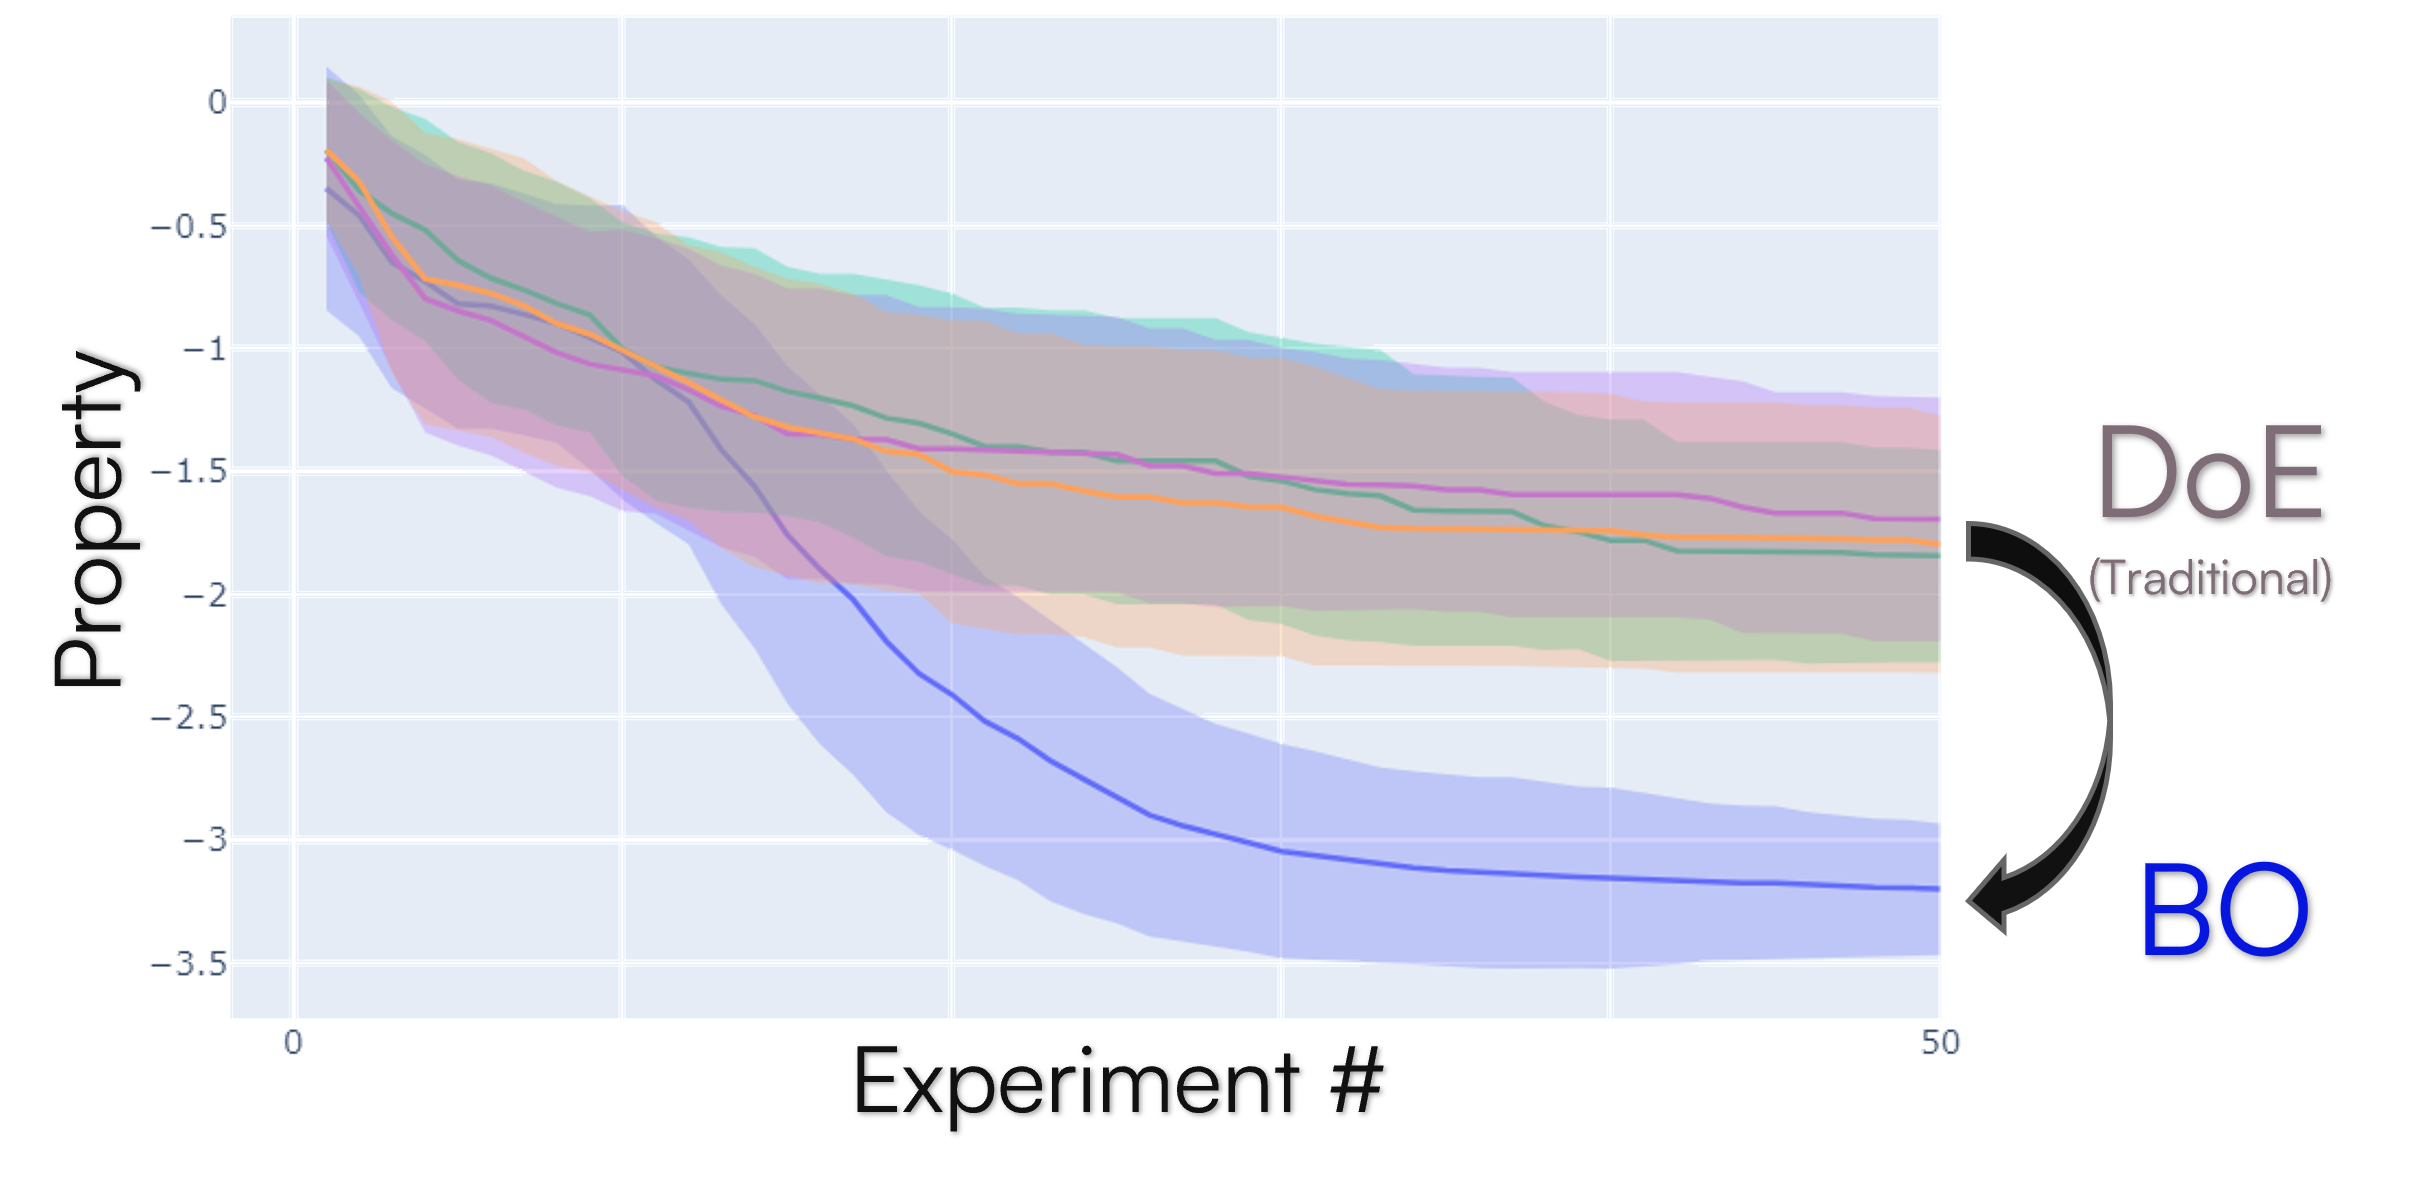
\includegraphics[width=1\linewidth]{latex/figures/intro-bo.png}
    \caption{Optimization traces for traditional design of experiment (DoE) methods compared with Bayesian optimization (BO), typically outperforms. BO uses a smart model to predict where to look next in an experiment to find the best results with few experiments.}
    \label{fig:intro-bo}
\end{figure}


The goal of the AC BO Hackathon was to leverage the expertise of a diverse, global community to advance the development and application of BO techniques for solving critical challenges in the physical sciences. The hackathon also aimed to foster collaboration and knowledge sharing among participants from different backgrounds, including academia, national laboratories, government agencies, and private industry. The event attracted 120 active participants from 44 teams, representing 41 academic institutions, 12 national labs, and 9 companies. Likewise, the participants were located in 38 cities, 14 countries, and 4 continents (\cref{fig:map}). A full list of projects, including links to the corresponding GitHub repositories, submission video, and social media post are provided in \cref{tab:projects}.

\begin{figure}[h!]
    \centering
    % \captionsetup{justification=centering}
    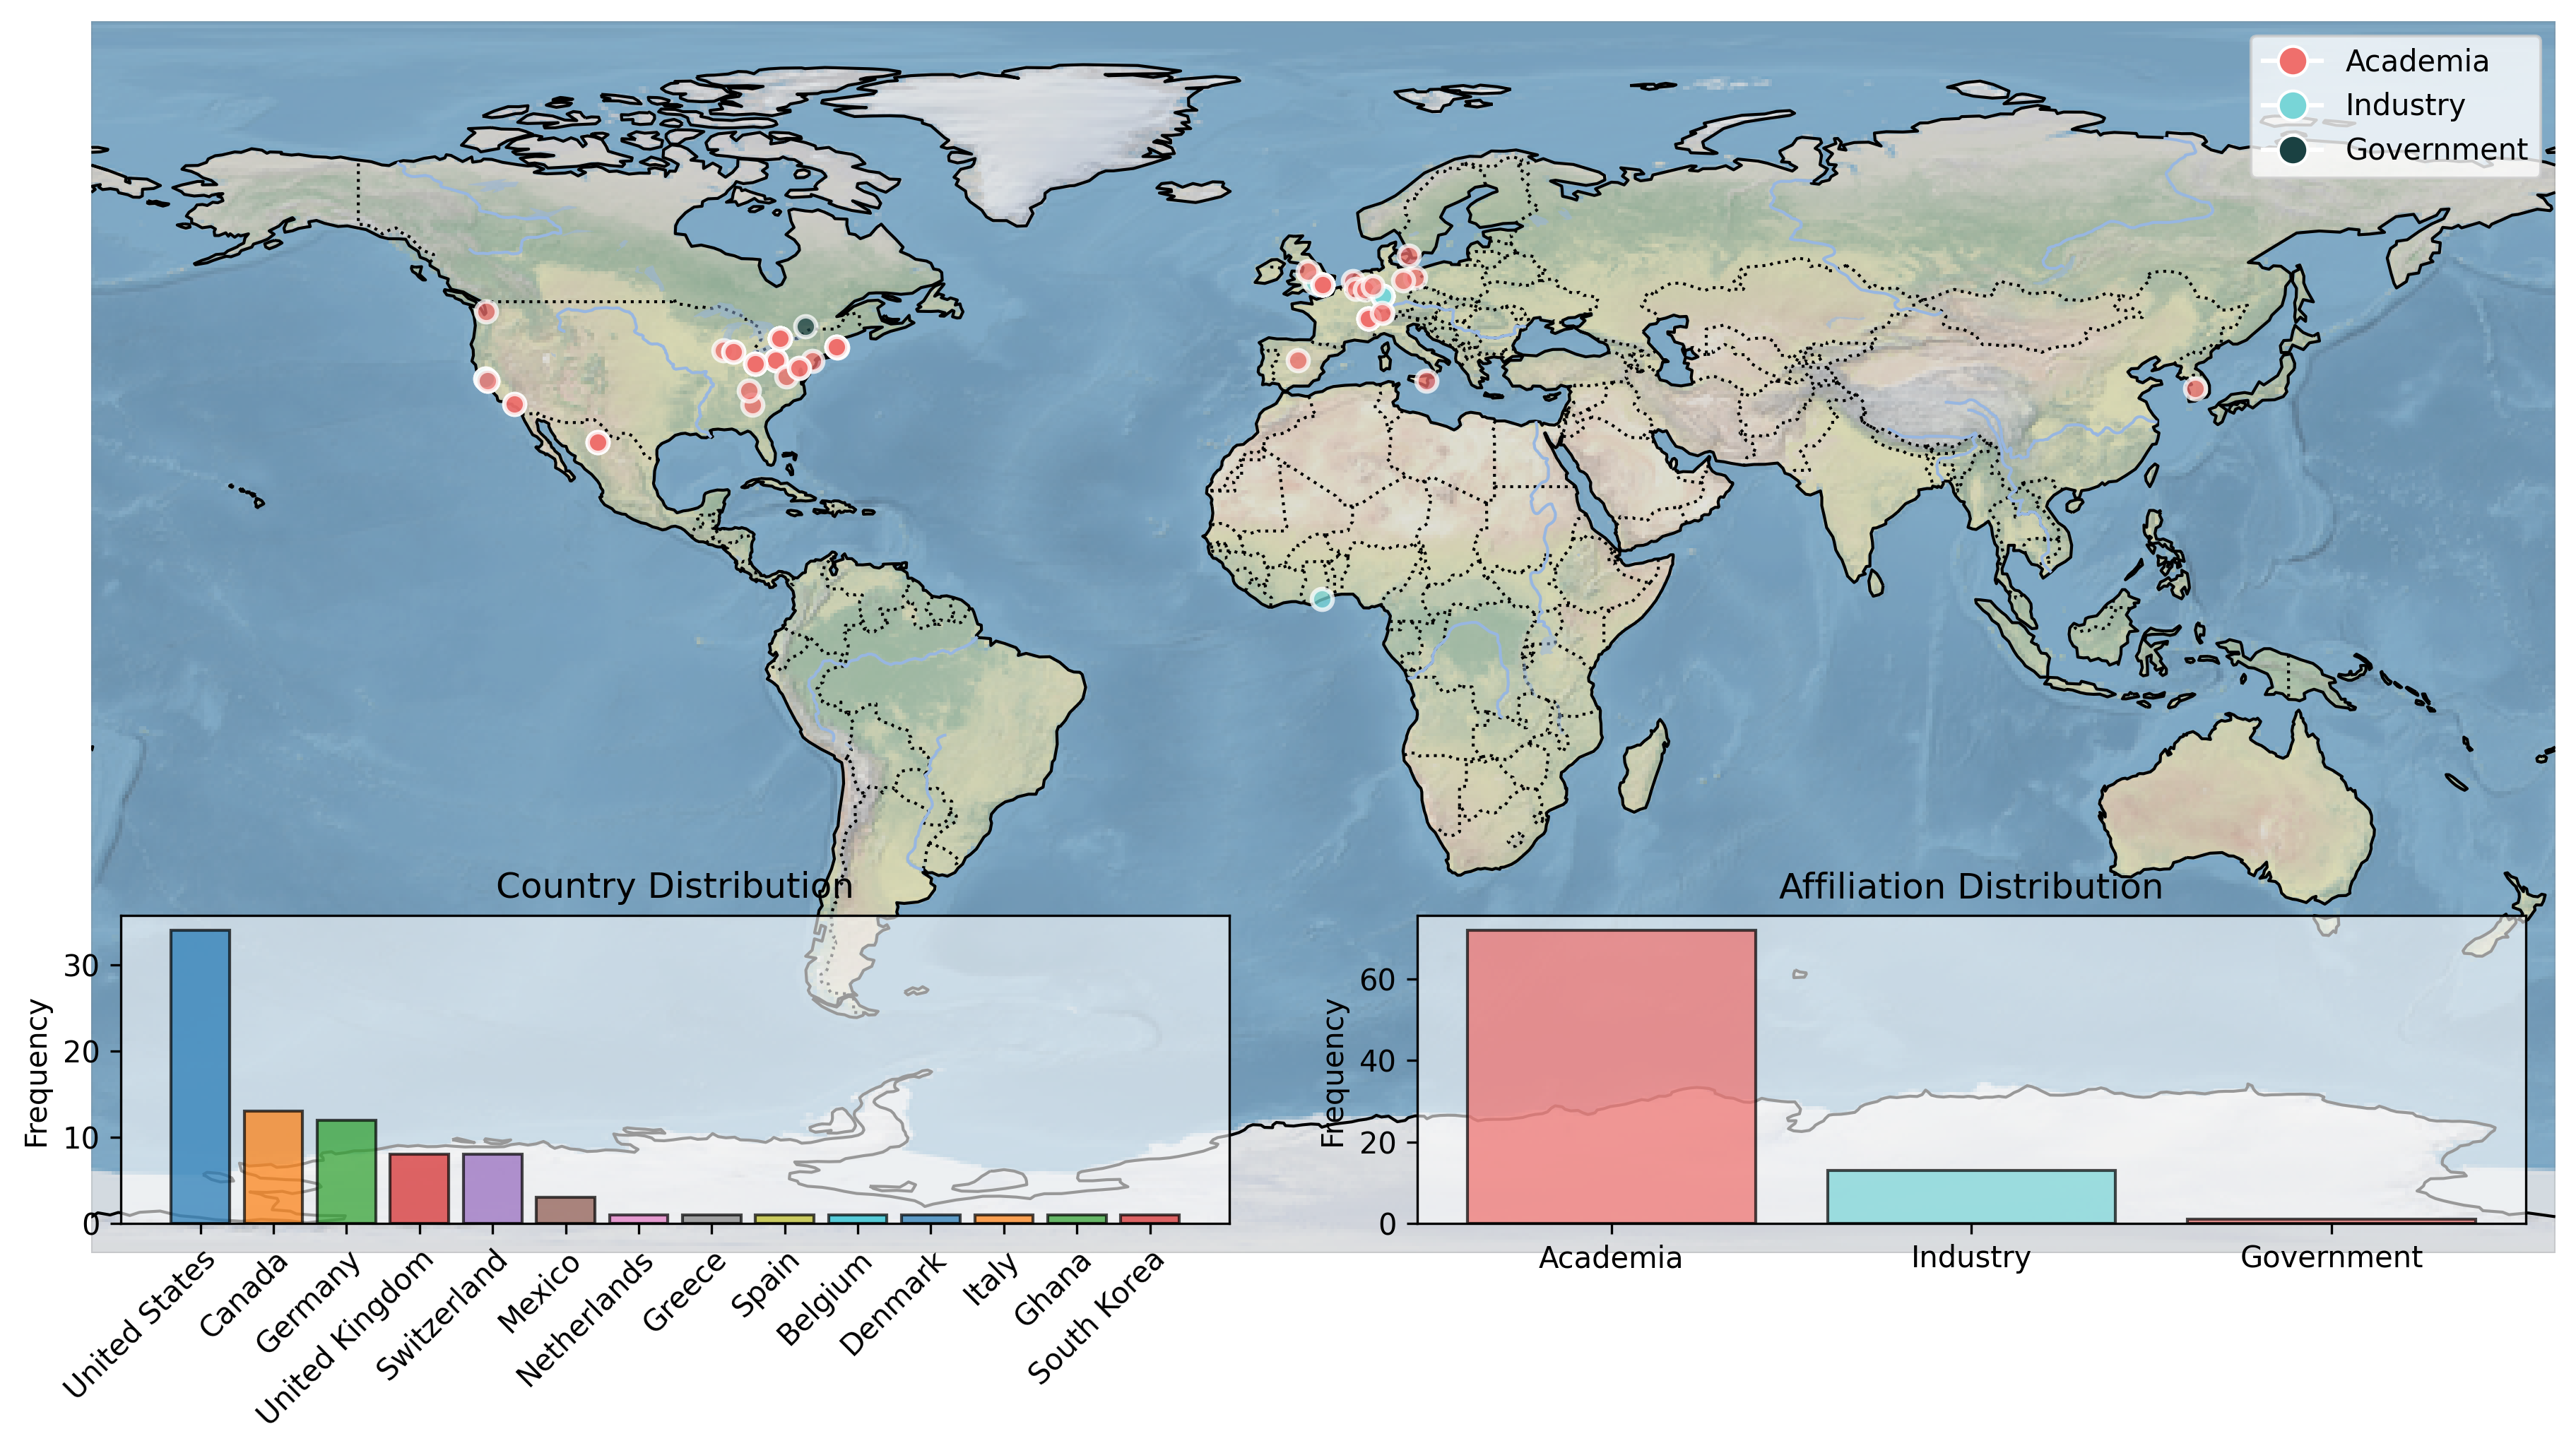
\includegraphics[width=1\linewidth]{latex/figures/world_map.png}
    \caption{Demographic distributions of the participating teams and their affiliations. \label{fig:map}}
\end{figure}

\begin{table*}[]
\caption{List of projects and project types, with links to corresponding website project pages, repositories, videos, and social media posts.}
\label{tab:projects}
\setlength{\extrarowheight}{0.4em}
\begin{tabularx}{\textwidth}{>{\centering\arraybackslash}p{1cm} X >{\centering\arraybackslash}X}
\toprule
\# & Project Name & Links \\ \midrule
\href{https://example.com}{\#1} & Project A & 
\href{https://github.com/example}{\faGithub} \,
\href{https://youtube.com}{\faVideo} \,
\href{https://twitter.com}{\faTwitter} \tabularnewline
\href{https://example.com}{\#2} & Project B & 
\href{https://github.com/example}{\faGithub} \,
\href{https://youtube.com}{\faVideo} \,
\href{https://linkedin.com}{\faLinkedin} \tabularnewline
\href{https://example.com}{\#3} & Project C & 
\href{https://github.com/example}{\faGithub} \,
\href{https://youtube.com}{\faVideo} \,
\href{https://twitter.com}{\faTwitter} \tabularnewline
\bottomrule
\end{tabularx}
\end{table*}


Participants were provided with various resources to prepare for the hackathon – this included GitHub classroom assignments with automated feedback, application- and theory-focused videos and tutorials, Python refresher materials, and a list of tools to consider using during the hackathon (\cref{fig:preparation}).

\begin{figure}
    \centering
    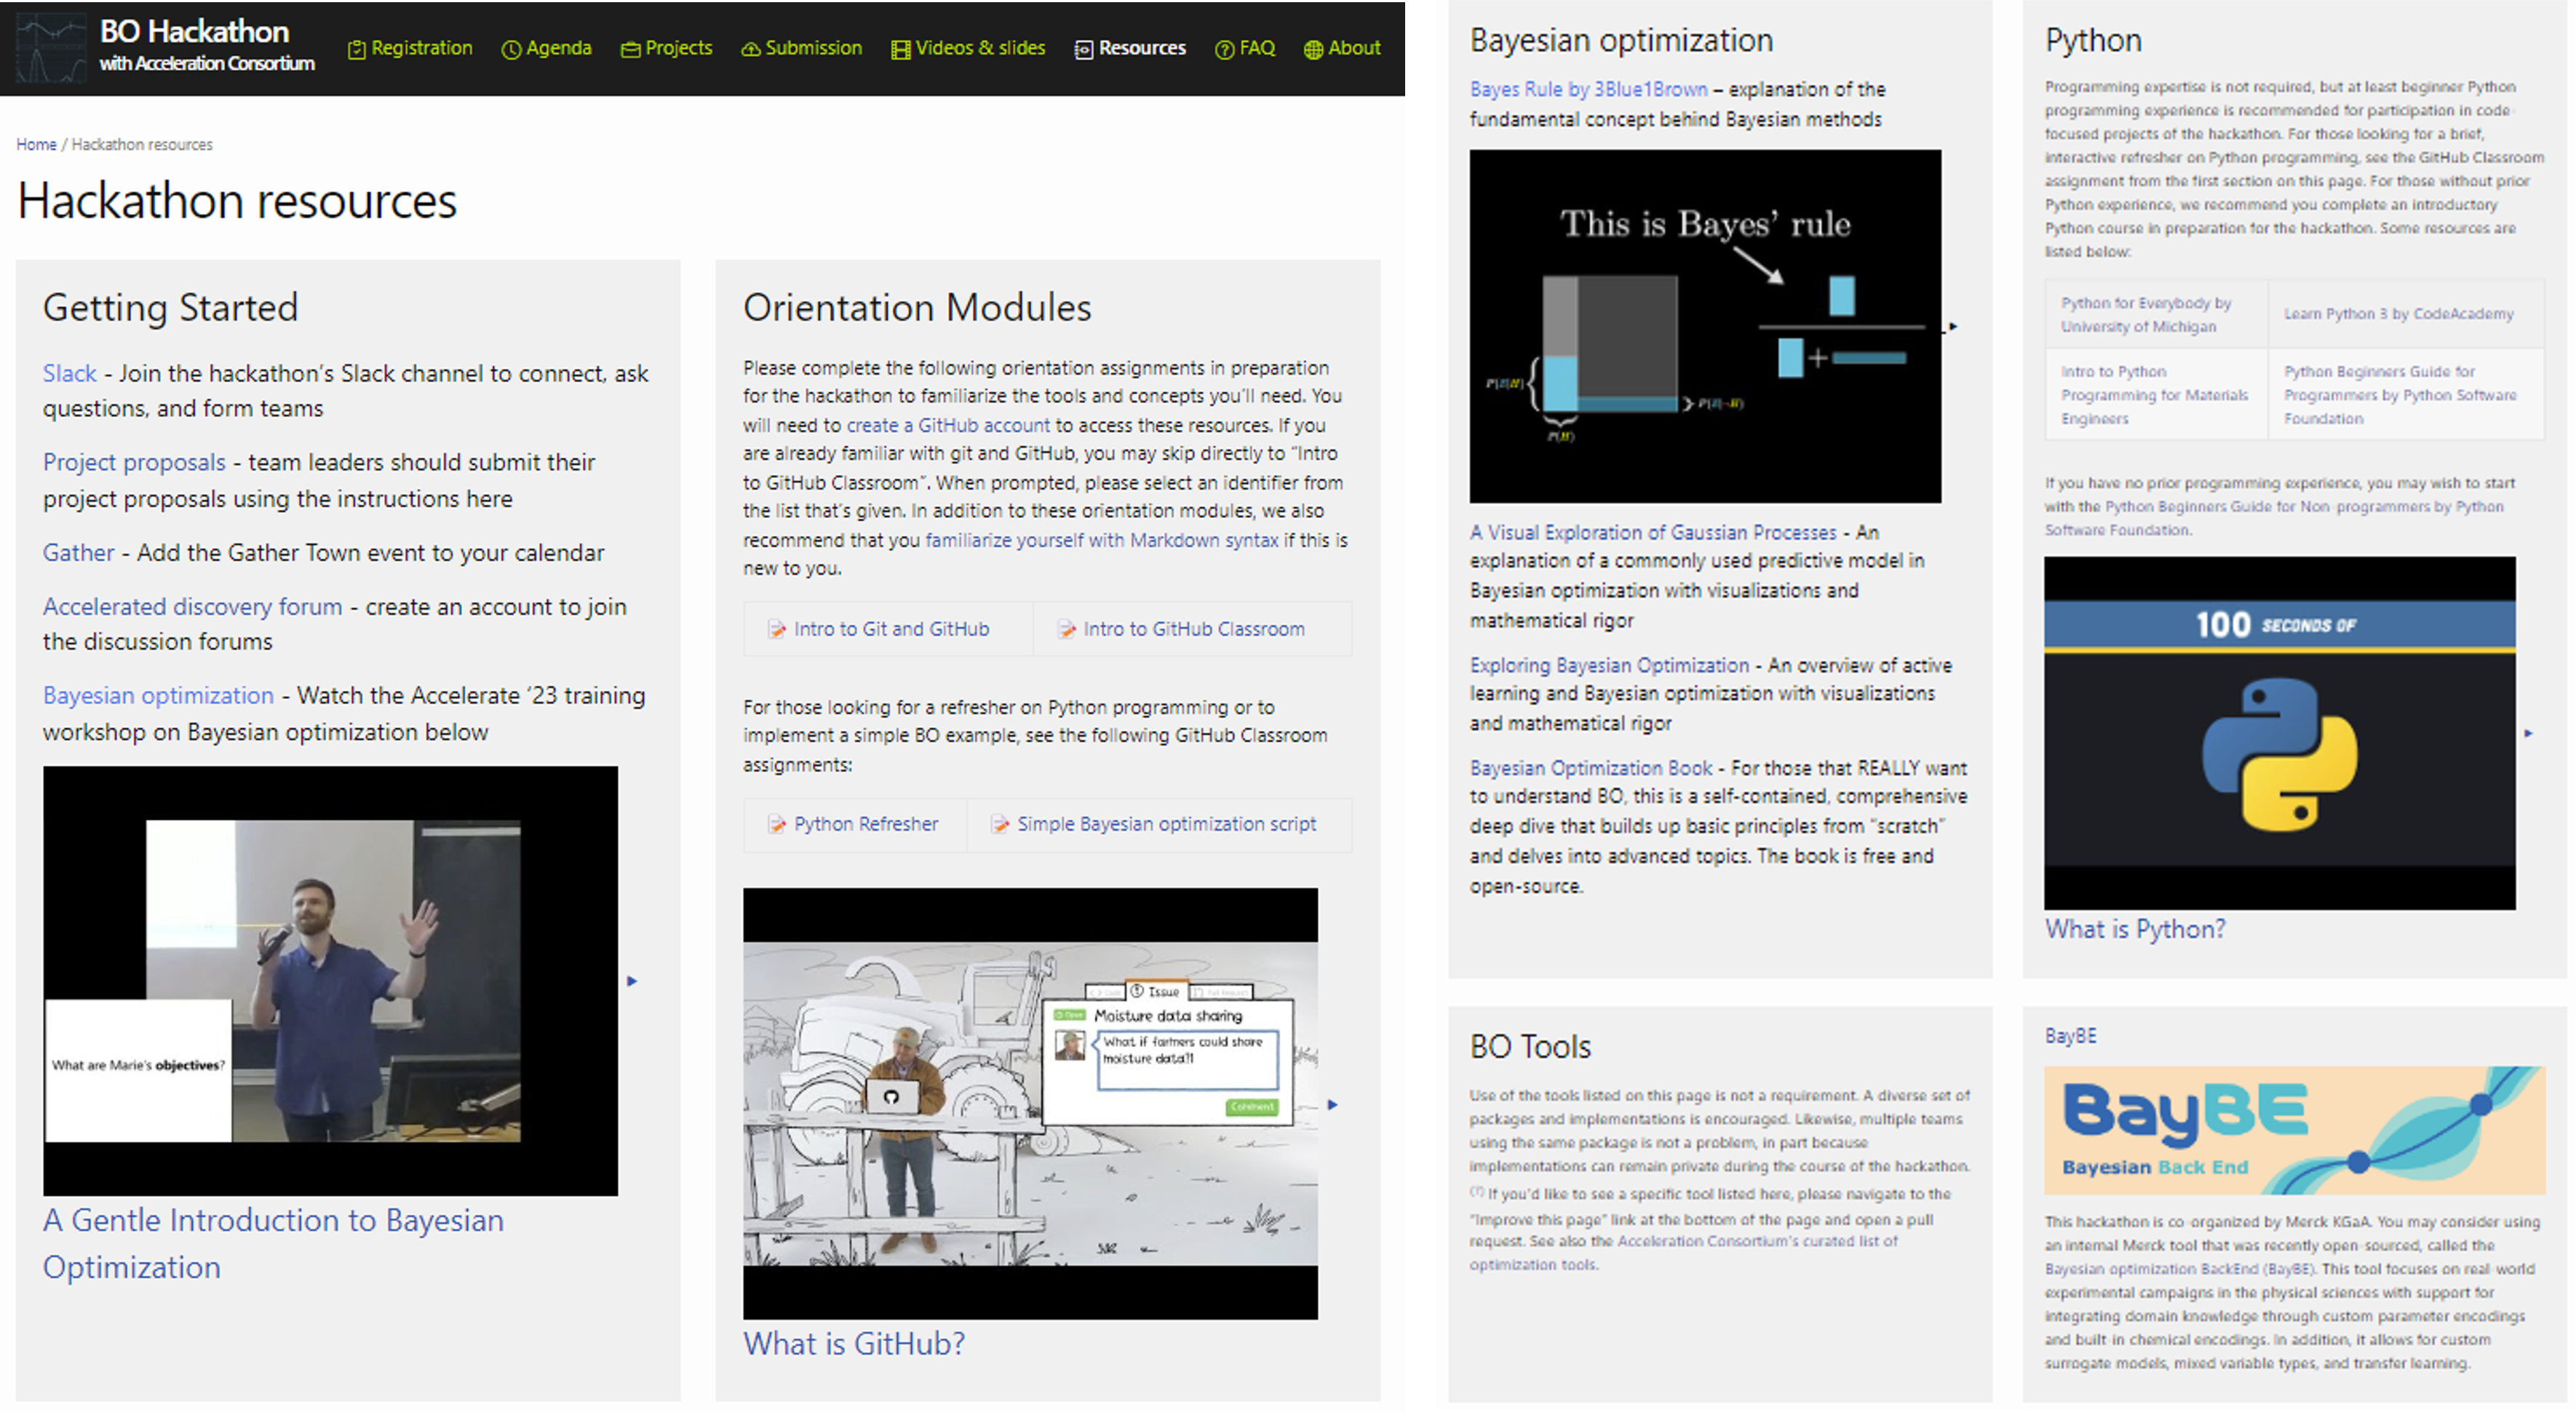
\includegraphics[width=1\linewidth]{latex/figures/preparation.png}
    \caption{A snapshot of \href{https://ac-bo-hackathon.github.io/resources/}{resources listed on the hackathon webpage} such as hackathon orientation, intro to BO, and Python refreshers.}
    \label{fig:preparation}
\end{figure}

One of the unique aspects of this event is that it was hosted in Gather Town, a sort of union between traditional video conferencing software and retro arcade-style avatars and virtual spaces (\cref{fig:gathertown}). Participants create a custom avatar and maneuver in a two-dimensional space. The videos and audio of other participants appear and become audible when nearby, and fade out when far away, simulating an in-person experience. At the beginning of the hackathon, all participants gathered to listen to keynotes in realtime, which were broadcasted via YouTube live and embedded into the Gather Town space. The videos were then \href{https://ac-bo-hackathon.github.io/videos-slides/}{made available on the hackathon website}. After 2 months, the videos collectively had approximately 1600 views. After the keynotes, teams were assigned tables in breakout rooms, each with a whiteboard. Individual tables were assigned as "private spaces" which isolated the shared audio and video within each space. This had a number of advantages for collaboration within and across teams.

\begin{figure}
    \centering
    \includegraphics[width=1\linewidth]{latex/figures/gathertown.png}
    \caption{Gather town \href{https://ac-bo-hackathon.github.io/videos-slides/}{keynote} room (left), custom avatars (top-right), and an example of a breakout room for teams (bottom-right). Keynotes were broadcasted in realtime to participants via an embedded YouTube livestream. Use of Gather Town leveled the playing field for teams who were in physically separate locations and made it easier for facilitators and other teams to have more natural "check-ins" with other projects.}
    \label{fig:gathertown}
\end{figure}


The hackathon concluded with a project showcase accompanied by crowdsourced judging within a "poster room" (\cref{fig:poster}).



% Preparation for the hackathon - 111 GitHub Classroom assignments accepted

% The hackathon was designed with tips, trick, and resources from various sources, such as https://github.com/github/hackathons.


% Hosts: Acceleration Consortium, Merck KGaA



\begin{table*}[]
\caption{Project Topics for the Hackathon. See \href{https://ac-bo-hackathon.github.io/submission/}{the submission page} for more details.}
\label{tab:project_topics}
\setlength{\extrarowheight}{0.4em}
\begin{tabularx}{\textwidth}{>{\centering\arraybackslash}p{0.5cm} p{4.5cm} X}
\toprule
 & \textbf{Topic} & \textbf{Description} \\ \midrule

1 & \textbf{Apply Algorithms} & Choose a package or algorithm and apply it to one of \href{https://huggingface.co/collections/AccelerationConsortium/optimization-benchmarks-66a44daf10de1a0335f28826}{the benchmark tasks prepackaged for the hackathon}. \\

2 & \textbf{Develop Benchmarks} & Develop a new benchmark and add it to the suite of benchmarks from above. \\

3 & \textbf{Create Tutorials} & Create "gentle introduction" tutorials for \href{https://ac-microcourses.readthedocs.io/en/latest/courses/data-science/overview.html}{advanced optimization topics}. \\

4 & \textbf{Propose Tasks} & Propose materials tasks that \textit{can} and \textit{should} be tackled with BO \\

5 & \textbf{General} & Other projects that are related to Bayesian optimization for the physical sciences \\

\bottomrule
\end{tabularx}
\end{table*}












\section*{Acknowledgements}

%\printglossaries

% \bibliographystyle{achemso}
\bibliography{latex/ac-bo-hackathon}

\end{document}